\chapter{Background}
\label{chap:background}

%---
\section{Chapter Overview}

In Chapter~\ref{chap:introduction}, the medical image segmentation and feature identification problems were introduced, and my thesis was formally stated. This chapter surveys the wide variety of segmentation and feature identification techniques currently in use in the field, with the intention of providing the background necessary to place the specific techniques I used for my own work in context. It also surveys existing work on the use of partition trees in the imaging domain. This background lays the foundation for Chapter~\ref{chap:methodology}, in which the research approach I chose is discussed in the context of the overall goals of my doctoral work.

Whilst the segmentation and feature identification problems are theoretically distinct -- in that feature identification involves assigning semantic meaning to parts of an image where segmentation does not -- there is a great deal of overlap between them in practice. For example, the goal of some of the segmentation techniques we will see (e.g.~region growing) is to directly segment a particular feature of interest; in that sense, they are as much feature identification approaches as segmentation ones. For that reason, I have chosen to present the techniques used for both problems together, rather than separately, commenting on the extent to which they address each of the problems where I feel it is appropriate.

%---
\section{Segmentation and Feature Identification Techniques}

\subsection{Overview}

The majority of the segmentation techniques in current use can be divided into eight classes: (1) thresholding techniques, which seek to segment an image based on dividing up the histogram of its grey values, (2) region growing techniques, which search for specific features by flooding outwards from one or more initial seed points in the image, (3) morphological techniques such as the watershed transform, which treats an image as a height map and divides it up into catchment basins that we try to ensure correspond to features of interest, (4) deformable models, which start with some arbitrary model of a desired feature and try to deform it to fit the image data, (5) learning techniques, which construct some variety of model based on a set of training images and use it to segment subsequent scans, (6) clustering techniques such as the K-means algorithm, (7) graph partitioning techniques such as the normalized cuts algorithm, and (8) hybrid techniques, which combine methods from the other classes to produce (what are hopefully good) results for specific applications. Each of these is discussed in more detail in one of the following subsections. The field as a whole is visually depicted in Figure~\ref{fig:background-segmentation-field}.

%---
\stufigex{height=16cm}{background/background-segmentation-field.png}{The field of image segmentation techniques}{fig:background-segmentation-field}{p}
%---

\subsection{Thresholding}

In principle, thresholding segmentation methods are quite simple. The idea is to divide the pixels of the image into classes through the use of one or more dividing lines on the image histogram. Dividing the image into two classes is known as \emph{binary thresholding}; where more classes are used, we refer to the process as \emph{multi-thresholding}. As an example, we could use binary thresholding to divide an 8-bit image (with grey levels ranging from $0 = \mbox{black}$ to $255 = \mbox{white}$) into two classes, one containing pixels greater than (say) $160$, and representing the foreground of the image, and the other containing all the remaining pixels and representing the background (see Figure~\ref{fig:background-thresholding-binaryexample}).

%---
% TODO: fig:background-segmentation-thresholding-binaryexample
\stufigex{width=16cm, height=9cm}{todo.png}{TODO}{fig:background-segmentation-thresholding-binaryexample}{p}
%---

The difficulty encountered in practice is how to determine the optimum threshold location(s). A misplaced threshold will cause an inaccurate segmentation, so choosing the location appropriately is essential. In our example above, choosing a threshold which was too high would mean that the foreground of the image would be \emph{undersegmented} (i.e. pixels which should be classified as being part of the foreground are incorrectly classified as background) and the background would be \emph{oversegmented} (the converse) -- see Figure~\ref{fig:background-segmentation-thresholding-inaccurate}(a). Choosing too low a threshold would cause the opposite problem -- see Figure~\ref{fig:background-segmentation-thresholding-inaccurate}(b).

%---
% TODO: fig:background-segmentation-thresholding-inaccurate
\begin{stusubfig}{p}
	\subfigure[TODO]
	{
\includegraphics[height=8cm]{todo.png}}%
	%
	\hspace{4mm}%
	%
	\subfigure[TODO]
	{
\includegraphics[height=8cm]{todo.png}}%
\caption{TODO}
\label{fig:background-segmentation-thresholding-inaccurate}
\end{stusubfig}
%---

Owing to difficulties like this, applications are often designed so that thresholds can be chosen interactively by the user, but a great deal of work has also been done on automatically determining good threshold locations. As surveyed by Sezgin and Sankur in \cite{sezgin04}, there are six types of approach to the problem in current use:

\begin{enumerate}

\item \emph{Histogram shape-based methods.} These use shape properties of the histogram to find a good threshold. For instance, Rosenfeld's histogram concavity method, cited in \cite{lee.c92}, works by examining the difference between a histogram and its convex hull. A grey level at which the the height difference between the histogram and its convex hull is greatest (i.e. a point of deepest concavity) is picked as the threshold value.

\item \emph{Clustering-based methods.} These try and group the grey level data into a given number of clusters (two in the case of binary thresholding). One example is the method of Ridler and Calvard \cite{ridler78}. Their idea was to take a grey-level image and produce an initial binary classification which makes the assumption that the object of interest is somewhere in the middle of the image and the corners of the image contain only background. The means of the pixels currently classified as background and object are calculated and the average of the two means is taken. The new value is then used to threshold the image and produce a new binary classification into background and object classes: it is assumed that this will be more accurate than the initial guess. Finally, the process is iterated until there is little or no change in the binary classification, and the last threshold in the iteration is chosen for use.

\item \emph{Entropy-based methods.} These are based on information theory and pick thresholds by (for example) trying to maximise the information content in the thresholded image. As described by Wong and Sahoo in \cite{wong89}, the simplest possible method looks at two probabilities, $F(T)$ and $F^*(T) = 1 - F(T)$, each parameterised in terms of a threshold, $T$. The first, $F(T)$, gives us the probability of a given pixel having a grey value less than or equal to the threshold, and the second, $F^*(T)$, gives us the probability of the value being greater than it. The information content in the thresholded image is given by
%
\[
H(T) = -F(T) \log_2 F(T) - F^*(T) \log_2 F^*(T)
\]
%
and attains a maximum when $F(T) = 0.5$. This is equivalent to saying that in the absence of any other knowledge, the maximum entropy principle tells us that the information contained in the thresholded image is maximised by picking a threshold which classifies half the pixels as background and half as foreground. This makes intuitive sense, but is too simplistic an approach for the majority of applications. Better alternatives have been developed, but are beyond the scope of this dissertation (TODO: this was appropriate for my transfer report, but not for my actual thesis).

\item \emph{Object attribute-based methods.} These pick thresholds based on a comparison between the original grey-level image and the binarized (i.e.~segmented into two classes) version of it. For example, the method of Hertz and Schafer \cite{hertz88} picks the threshold that yields a binarized image whose edge field maximally corresponds to that of the original image. The edge fields in this case are obtained via the well-known Sobel operator \cite{gonzalez02}.

\item \emph{Spatial methods.} An example of a spatial thresholding method is Wu et al.'s approach in \cite{wu82}. This first constructs a quadtree from the image by splitting image regions until they have a low standard deviation (where they define `low' in terms of the standard deviation of the image as a whole). This divides the image into square blocks of various different sizes. The observation is that the smaller blocks tend to be near the boundaries between foreground and background in the image -- the quadtree can thus be used as a way of estimating where these boundaries are. Having classified the pixels in the image in this way, it is possible to construct a histogram of the grey values of non-boundary pixels in the image, which it is hoped will be more bimodal than the histogram of the grey values in the image as a whole. A threshold can then be placed at the deepest point in the value between the two modes. Alternatively, a histogram of the boundary pixels can be constructed, which it is hoped will be unimodal, and a threshold can be placed at the mean of this histogram instead.

\item \emph{Local / adaptive methods.} These vary the threshold for each pixel location in the image. Two examples of this are the methods of Bernsen \cite{bernsen86} and Niblack \cite{niblack86}. As described by Trier and Jain in \cite{trier95}, Bernsen's method takes the highest and lowest grey values, $g_{\mbox{max}}$ and $g_{\mbox{min}}$, in a suitably-sized window around each pixel, and uses them to calculate a contrast measure $C = g_{\mbox{max}} - g_{\mbox{min}}$. If $C$ is less than some user-specified value, the local neighbourhood around the pixel is taken to be uniform, and an appropriate choice is made about whether the pixel should be classified as background or foreground (in \cite{trier95}, pixels were always classified as background in this case). Otherwise, a threshold value $T = (g_{\mbox{max}} + g_{\mbox{min}}) / 2$ is calculated, and the pixel is classified as foreground if its value is greater than $T$, and background if not. Niblack's method, by contrast, bases its decision on the mean and standard deviation of the grey values in the local neighbourhood around a pixel. In particular, if $m$ is the local mean and $s$ the local standard deviation, Niblack's method calculates a local threshold $T = m + ks$, where $k$ is a (negative) user-specified parameter. Again, a pixel is classified as foreground iff its grey value is greater than $T$.

\end{enumerate}

\noindent In spite of the large amount of work done on thresholding, however, it has some significant downsides when used on its own to process medical images:

\begin{itemize}

\item It divides the image into two or more groups of pixels, based on their grey values, but there is no guarantee (or even an expectation) that any of these groups will be contiguous in the image. For instance, trying to segment a kidney from a CT scan by bounding it between two grey value thresholds might also result in inadvertently segmenting blood vessels across the image as well (their grey levels are quite similar to those of the kidneys). Not only are these blood vessels not part of the kidney, they are actually physically separated from it in the image! (It is also worth noting that trying to segment a kidney will generally result in segmenting both of them at once, since their grey level ranges are the same. This sort of problem can be overcome by specifying the side of the body in which we're interested.)

\item It is by no means the case that acceptable threshold locations always exist. If the grey value ranges of different objects of interest significantly overlap, it may be impossible to separate them using thresholding alone.

\end{itemize}

\noindent These limitations can in some cases be overcome by combining thresholding with other techniques. For instance, the results of thresholding often have gaps in them, which can sometimes be filled in by carefully applying various morphological operators (e.g. morphological opening and closing). Luc Soler's team \cite{soler01} made use of thresholding (as one technique among many) and achieved excellent automatic segmentation results for the liver. However, they did not use thresholding on its own. For instance, they segmented bones by thresholding for bright areas and then keeping only those which were near to the fat tissue (which had already been segmented). Simple thresholding alone would have been insufficient for the task, since structures such as the aorta also appeared bright on the contrast-enhanced images.

\subsection{Region Growing}

Region growing methods for segmentation essentially work as follows. First, an initial seed point is chosen for a feature of interest. Then, the region is `grown' by iteratively considering all points which are adjacent to the region and adding any which satisfy certain criteria. For example, we could choose to add adjacent pixels whose grey value differs from that of their neighbour in the region by less than a certain amount. Alternatively, we could try and add adjacent pixels which preserve the homogeneity of the entire region (for some suitable definition of homogeneity). A basic region growing algorithm can be implemented straightforwardly using a queue. Starting from a queue containing only the initial seed point, we repeatedly pop the pixel at the front of the queue, consider its non-region neighbours for addition to the region, and push any which satisfy the requisite criteria onto the end of the queue. The process terminates when the queue empties.

The key issues when implementing region growing are how to choose the seed point, how to formulate the criteria specifying which points to add to the region, and how to decide when the process should terminate. For automated segmentation methods, how to choose the seed point is of fundamental importance; semi-automated algorithms can focus exclusively on the latter two problems, relying instead on the user to interactively specify an initial seed.

As mentioned above, one of the simplest approaches to region growing is to add adjacent pixels which are within a certain fixed threshold value of their neighbour in the region. Practical region growing methods, however, such as \cite{lin06,pohle01}, tend instead to use \emph{adaptive} region growing, whereby the criterion varies to take account of the area around the pixel under consideration. In \cite{lin06}, for example, the approach taken is as follows. After locating an initial seed point $(s_x, s_y)$, a $7 \times 7$ mesh is placed over it and the maximum and minimum pixel intensities within the mesh, $M(s_x, s_y)$ and $m(s_x, s_y)$ are determined. From these, a contrast range $t_0 = M(s_x, s_y) - m(s_x, s_y)$ is calculated and recorded. Next, for each pixel $(x,y)$ under consideration for addition to the region, values $M(x,y)$ and $m(x,y)$ are similarly calculated, and a local value $\theta_{\rm local} = (M(x,y) + m(x,y)) / 2$ is determined. The region growing criterion is then formulated as $|f(x,y) - \theta_{\rm local}| \le t_0$, i.e. we add an adjacent pixel $(x,y)$ to the region if the absolute difference between its grey value $f(x,y)$ and the midpoint of the contrast range of the $7 \times 7$ mesh surrounding it is less than the contrast range of the $7 \times 7$ mesh centred on the initial seed point. The region growing is specified to stop when this absolute difference is greater than a certain threshold, implying that the area surrounding a given pixel is not homogeneous.

The advantages of region growing methods are that the resultant region is guaranteed to be connected in the image (unlike with thresholding) and that they are, on the whole, fairly easy to implement. However, from the point of view of automatic segmentation, they present difficulties, because choosing an initial seed point is in general a non-trivial problem. The usual approach taken for automatic seed point selection is to rely on statistical data about where the features of interest (e.g. organs) usually lie in the body. For instance, the approach in \cite{lin06} is to search for suitable seed points in two elliptical regions on each side of the body, one for each kidney. This works quite well, but doesn't seem as if it would be that robust if tested on unusual cases.

Whilst region growing algorithms are guaranteed to produce a connected result, the region may still have holes in the middle of it. Whilst this may be desirable if we really are trying to segment a torus-shaped feature, on the whole we need to post-process the region growing results to remove these holes. Common techniques for doing this include morphological closing, etc.

\subsection{Morphological Techniques}

Mathematical morphology is a large and rather general field based on lattice theory \cite{?}. It contains many useful image processing techniques, the majority of which are not relevant for the purposes of this survey, but in segmentation terms its key technique is the watershed transform, originally developed by Serge Beucher \cite{beucher90}.

The watershed, which will be described in substantially more detail in Chapter~\ref{chap:segmentation}, is essentially a technique for dividing landscapes into their catchment basins (where a catchment basin is an area of the landscape from which water would run down to a given local minimum). In imaging terms, this can be utilised for segmentation purposes by treating an image as a discrete landscape and pre-processing it so as to try to establish a correspondence between catchment basins in the landscape and features of interest in the image. If such a correspondence can be successfully established, finding the catchment basins then equates to finding the desired image features.

Many image algorithms have been developed to actually perform the watershed transform; in general, these can be classified as either flooding algorithms (e.g.~\cite{bieniek00,rambabu07}) or rainfalling algorithms (e.g.~\cite{meijster98,osma-ruiz06,stoev00}). The former essentially flood out from the local minima in the landscape and (implicitly or otherwise) add watershed boundaries where the different catchment basins meet; the latter determine paths of steepest descent from points in the landscape and assign them to catchment basins based on the local minima to which their paths lead down.

In practice, however, it is rarely possible to establish a perfect correspondence between the catchment basins in the landscape and the desired features in the image, as to do so consistently would require prior knowledge of where the desired features actually are in the image, which would defeat the point of segmenting the image in the first place. One of the most common problems encountered with the watershed transform is that of oversegmentation: the landscape fed into the watershed has an excess number of catchment basins, most of which do not correspond to anything of interest in the actual image. This is particularly true of landscapes representing noisy images -- small changes in grey values can create shallow catchment basins, or dimples, in the landscape, greatly affecting the resulting segmentation.

There are two main approaches in the literature for dealing with this problem, namely marker imposition (leading to an approach known rather aptly as `watershed-from-markers') and hierarchical segmentation. Marker imposition essentially works by specifying markers on particular features of interest a priori, and flooding out only from those. This partitions an image into a number of regions equal to the number of specified markers and thereby solves the oversegmentation problem. Unfortunately, it can be extremely difficult to determine the required markers automatically -- rather than solving the underlying problem, we have merely changed it into one of marker determination. This may or may not prove problematic, depending on the data available and the specifics of the application. In some cases, it may be possible to use other data to determine marker placement automatically -- for example, Grau et al.\ \cite{grau04} successfully used a statistical atlas for this. In other cases, it may simply be acceptable to place the markers manually \cite{xue05}, or to initially place them manually and then propagate them from one image in a sequence to the next \cite{flores09}.

In situations where neither is the case, however, the alternative approach of hierarchical segmentation can be used. As one might expect, the general idea here is to take the oversegmented result of running the watershed transform on an image, and perform several iterations of region merging to produce a hierarchy of gradually coarser partitions of the original image. As will be illustrated in far more detail in Chapter~\ref{chap:segmentation}, this is exactly the sort of approach taken by the waterfall transform \cite{beucher90,marcotegui05}: what is unique about the waterfall, however, is that each of its iterations in which it merges regions together is itself a watershed transform.

As will be discussed in Chapter~\ref{chap:methodology}, the hierarchical approach to watershed segmentation is interesting for a couple of reasons: on the one hand, it produces, without requiring a great deal of manual fine-tuning, segmentations which, whilst not perfect, are often quite reasonable to a first approximation; on the other hand, the hierarchy of partitions of the image it produces can be turned into a tree structure (see \S\ref{sec:background-partitiontrees}) which is amenable to further editing, allowing any flaws in the initial segmentation to be corrected in an intuitive manner. These two qualities make this approach eminently suitable in situations where automated solutions are desirable but interactive control remains important.

\subsection{Deformable Models}

As their name suggests, deformable models methods work by taking an initial model of the features under consideration and deforming it to fit the actual data available. The initialisation of the model is generally based on \emph{a priori} anatomical knowledge. The model itself can be represented in a variety of ways, and these ways correspond to a number of different approaches to the problem. For example, the snakes method, which we will see shortly, represents the model as a parametrically-defined spline, and is hence referred to as an example of a parametric deformable model (it is sometimes also referred to as an explicit deformable model). In contrast, level sets represent the model \emph{implicitly} and are an example of implicit deformable models. Implicit deformable models were developed later than their parametric counterparts, but both types see a lot of use.

\subsubsection{Parametric Deformable Models}

\paragraph{Snakes}

As originally defined by Kass, Witkin and Terzopoulos in \cite{kass88}, `A snake is an energy-minimizing spline guided by external constraint forces and influenced by image forces that pull it toward features such as lines and edges.'

Essentially, the idea works as follows. We represent the position of the snake, in terms of a spline parameter $s$, as $\mathbf{v}(s) = (x(s),y(s))$, and define an \emph{energy functional}, $E_{snake}^*$, as
%
\[
E_{snake}^* = \int_0^1 E_{int}(\mathbf{v}(s)) + E_{image}(\mathbf{v}(s)) + E_{con}(\mathbf{v}(s)) \; ds.
\]
%
The three terms in the summation are \emph{internal} energy, which tries to limit the curvature of the snake, \emph{image} energy, which tries to attract the snake towards features in the image such as lines and edges, and \emph{constraint} energy, which allows the user to apply constraints to influence the result of the segmentation. The snake algorithm as a whole attempts to find a spline minimising $E_{snake}^*$.

The original snakes paper describes a continuous model, but more recent research \cite{lobregt95,miller90b,miller90a} has seen the development of discrete models as well. The model described by Lobregt and Viergever in \cite{lobregt95}, called a \emph{discrete dynamic contour model}, is particularly interesting, and worth describing in more detail. Rather than relying on ideas of energy-minimization, Lobregt and Viergever model snakes using a force-based physical simulation. In their approach, a snake is a set of vertices connected by edges. At each time-step, various forces are applied to each vertex, which gradually \emph{deform} the snake towards the desired result. The results of this approach will depend to an extent on the lengths of the edges joining the vertices: if an edge is too long, important image features may pass through the gaps between vertices; if it is too short, the snake may become overly fixated on small details, not to mention the speed of the process being adversely affected. For this reason, after each deformation step, the snake is \emph{resampled} (by adding or removing vertices where necessary) to keep the edge lengths within certain limits.

The forces applied to each vertex closely mimic the energy terms in the original snakes paper. The force $\mathbf{f_i}$ applied to vertex $i$ is defined as the weighted sum
%
\[
\mathbf{f_i} = w_{ex}\mathbf{f_{ex,r_i}} + w_{in}\mathbf{f_{in,i}} + \underbrace{w_{damp}}_{< \; 0}\mathbf{v_i},
\]
%
where $\mathbf{f_{ex,r_i}}$ is an \emph{external} force term corresponding to the image and constraint terms from the original formulation, $\mathbf{f_{in,i}}$ is an \emph{internal} force term corresponding to the original internal term, and the remaining term is a new addition used to apply damping to try and bring the simulation to rest. (The real numbers $w_{ex}$, $w_{in}$ and $w_{damp}$ specify the weights to be given to each of these three factors. The paper tended to set all three of these to $0.5$: apparently this was derived empirically.)

It is important to mention that the method relies on quite a close initialisation (i.e.\ image features have quite a short capture range). In \cite{ree05}, this problem is circumvented by peforming a watershed-from-markers segmentation and using the result of that to initialise the snake. Another alternative, referred to there, is to try and add additional external forces to solve the problem: in particular, some success has been had with \emph{balloon forces} \cite{cohen91} and \emph{gradient vector flow} \cite{xu98}.

Problems of this kind with snakes methods have led to a great deal of interest in level sets as an alternative, although snakes also remain popular as a well-established and far simpler alternative. They also have the advantage that they can represent open structures as well as closed ones.

\paragraph{NURBS-Based}

Another type of parametric deformable model, this time based on non-uniform rational B-splines (NURBS), is described by Tsagaan et al.\ \cite{tsagaan02}, in which they use a 3D NURBS-based model of a kidney and deform it by minimizing an energy function. Their results seem good in some cases, but differ markedly from the manually segmented results they show in others.

\subsubsection{Implicit Deformable Models}

\paragraph{Level Sets}

Curves and surfaces in general can be specified either explicitly (such that they can be calculated directly from the definition) or implicitly (the opposite). For instance, an explicit (parametric) representation of a circle in terms of its radius $r$ and an angle $\theta$ might be:
%
\begin{eqnarray*}
x & = & r \cos \theta \\
y & = & r \sin \theta
\end{eqnarray*}
%
The corresponding implicit representation would be:
%
\[
x^2 + y^2 = r^2
\]
%
As we have seen, parametric deformable model approaches like snakes represent their model using the former approach. Level set approaches, by contrast, use the latter. As an introduction to the ideas behind level sets, consider the function $\psi(x,y) = x^2 + y^2$, which defines a scalar field over $\mathbb{R}^2$. For any value $k > 0$, the equation $\psi(x,y) = k$ defines a circle in the x-y plane: we will refer to each of these circles as an \emph{isosurface} of $\psi$, because each of them is the surface (curve) of all the points at which $\psi$ takes a particular value.\footnote{\emph{Iso} means `equal' in Greek, so here we are talking about the surface containing all the points with the same $\psi$ value.} The key idea is that if we now change $\psi$, for instance by redefining it as $\psi(x,y) = x^3 + y^3$, the isosurfaces change, in this case from circles to hypercircles. Thus by changing the function $\psi$, we can move the isosurfaces of $\psi$ around without ever having to represent them explicitly. Level set approaches make use of this by representing the deformable model as an isosurface of some function $\psi$, and then modifying $\psi$ to deform the model towards the boundary of the desired image feature.

%---
\stufigex{height=8cm}{background/background-segmentation-levelsets-circleexample.png}{A simple circular contour which gradually expands over time}{fig:background-segmentation-levelsets-circleexample}{p}
%---

%---
\stufigex{height=8cm}{background/background-segmentation-levelsets-ellipseexample.png}{An example of a contour which changes its shape over time}{fig:background-segmentation-levelsets-ellipseexample}{p}
%---

To represent contour changes over time, level set approaches make $\psi$ a function of time as well, and define it over some domain $U \subset \mathbb{R}^N$, giving us $\psi(\mathbf{x}, t) : U \times \mathbb{R}^+ \rightarrow \mathbb{R}$. They then set this equal to some constant (generally $0$) to actually specify one of the isosurfaces of $\psi$ as the contour being deformed. As a simple example of this, consider a circle, centred at the origin, which gradually expands outwards as the time increases (see Figure~\ref{fig:background-segmentation-levelsets-circleexample}). Supposing its radius to be $t$ at time $t$, we could represent this as:
%
\[
\psi((x,y),t) = x^2 + y^2 - t^2 = 0
\]
%
A more complicated example might involve gradually changing the circle into an ellipse over time (see Figure~\ref{fig:background-segmentation-levelsets-ellipseexample}). This could be achieved by writing:
%
\[
\psi((x,y),t) = x^2 + (yt)^2 - t^2 = 0
\]
%
Thus far, we have examined the basic ideas underpinning level sets, but not seen how they can be applied to the practical problem of segmentation. A common approach of real-world level set methods is to take as input not an explicit function of the kind we have just seen, but an initial contour on the image. This will then be deformed (using numerical methods) over time to try and fit it to an image feature of interest. There are thus six essential questions to consider:

\begin{enumerate}

\item How do we represent the function $\psi$?

\item Given an initial contour by the user, how do we use it to construct the initial function $\psi(\mathbf{x}, t = 0)$?

\item How do we define a numerical method to deform the initial function over time?

\item How do we know when the algorithm has terminated?

\item How do we extract the contour of interest over time?

\item How do we try and make the algorithm segment the desired image feature?

\end{enumerate}

To answer these questions, we consider the level set approach of Malladi et al., described in \cite{malladi95}. There, as tends to be the case for level set approaches in general, the function $\psi$ is represented by storing a discrete grid of approximate values over the domain $U$. The grid is uniformly-spaced, with squares of side $h$ (see Figure~\ref{fig:background-levelsets-grid}). Each grid node has (for each integer value of $n \ge 0$) an associated value $\psi_{ij}^n$, which approximates the value $\psi(ih,jh,n\dt)$, where $\dt$ is the time step of the numerical method that will be used to deform the initial contour over time.

% TODO: fig:background-levelsets-grid

The initial goal is to construct, from a contour specified by the user, the grid of values $\psi_{ij}^0$ approximating the function $\psi(\mathbf{x},0)$. In \cite{malladi95}, this is done by setting $\psi_{ij}^0$ to be the signed distance of the grid node $ij$ from the initial contour (points outside the contour are assigned positive values and those inside are assigned negative ones) -- see Figure~\ref{fig:background-levelsets-initialfunction}.

% TODO: fig:background-levelsets-initialfunction

Having constructed the grid for the initial function, the next step is then to define an appropriate numerical method to deform it over time. To do this, we first need a partial differential equation for $\psi$. The appropriate PDE, as derived in \cite{malladi95}, is:
%
\[
\pd{\psi}{t} + F|\nabla \psi| = 0
\]
%
Here, $F$ is called the \emph{speed function}, and will be used to control how $\psi$ evolves in a manner that will be discussed below. This can be approximated numerically as
%
\[
\frac{\psi_{ij}^{n+1} - \psi_{ij}^n}{\dt} + (F)(\nabla_{ij} \psi_{ij}^n) = 0,
\]
%
where (as noted, and described in more detail, in the paper), $\nabla_{ij} \psi_{ij}^n$ is `some appropriate finite difference operator for the spatial derivative'. This equation can be iteratively solved using standard numerical techniques \cite{?} and used to deform the model over time. The algorithm terminates when the contour of interest no longer changes between iterations.

To extract the contour of interest after each iteration, Malladi et al. construct a piecewise linear approximation to it, the gist of which involves finding the squares where some of the corner values are positive and some are negative, and constructing line segments therein. This bears not a little resemblance to the marching squares algorithm, the 2D analogue of marching cubes \cite{lorensen87}.

The remaining issue is how to use this algorithm to actually segment features in an image. For this, we make use of the speed function $F$, which controls how the contour deforms. Malladi et al.\ go into great detail about how $F$ should be defined, but essentially the idea is to define it so as to have (a) an advection component -- basically a term providing a constant speed inwards or outwards, (b) an image component -- a term which tries to make the contour move quickly when it is not near potential feature boundaries and slowly when it is close to them, and possibly (c) a geometry component -- a term which aims to control the local curvature of the contour. For the two-component version, with only an advection and an image component, this corresponds to an equation of the form
%
\[
\pd{\psi}{t} + (F_A + \hat{F}_I)|\nabla \psi| = 0,
\]
%
where $F_A$ is the advection component and $\hat{F}_I$ is the image component. For the version with a geometry component as well, the equation becomes
%
\[
\pd{\psi}{t} + \hat{k}_I(F_A + F_G)|\nabla \psi| = 0,
\]
%
where $F_G$ is the geometry component and $\hat{k}_I$ fulfils the role of the image component in the previous equation. The detailed definitions of the various components can be found in \cite{malladi95}. It is worth noting that this term-based approach bears a lot of similarity to that used for snakes, and in general the motivations for the various terms are more or less the same in each case.

Level sets have a number of advantages over snakes. One advantage is that they handle topological changes in an extremely simple fashion. For instance, consider Figure~\ref{fig:background-segmentation-levelsets-topologychanges}(a), in which the isosurface $\psi = 4$ is divided into two separate components. This is seamlessly represented by a level set approach, since it merely has to maintain a grid of numbers and not one or more explicit curves. Furthermore, the number of components can evolve over time without any special handling being required: in Figure~\ref{fig:background-segmentation-levelsets-topologychanges}(b), a change to the value of a single grid point can merge the two separate components into one, changing the topology at a stroke without any fuss. A corresponding implementation with snakes would involve far more work.

%---
\begin{stusubfig}{p}
	\subfigure[An isosurface divided into two separate components]
	{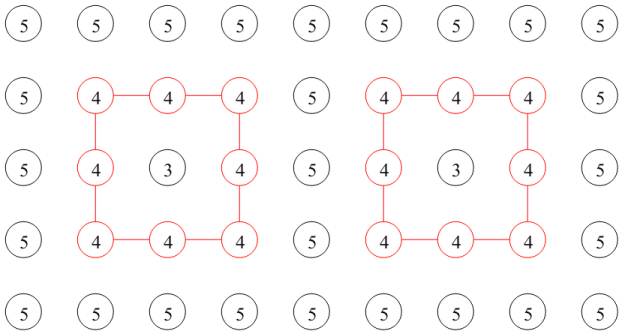
\includegraphics[width=.45\linewidth]{background/background-segmentation-levelsets-topologychanges-a.png}}%
	%
	\hspace{4mm}%
	%
	\subfigure[Changing a single grid value merges the two components into one]
	{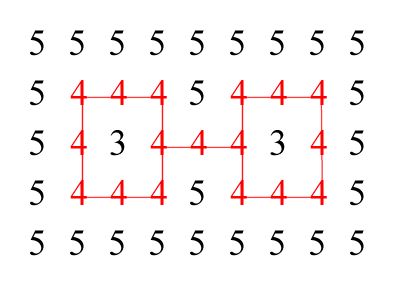
\includegraphics[width=.45\linewidth]{background/background-segmentation-levelsets-topologychanges-b.png}}%
\caption{Level set approaches seamlessly handle multiple boundaries and changes in topology}
\label{fig:background-segmentation-levelsets-topologychanges}
\end{stusubfig}
%---

Another advantage of level sets is that, unlike snakes, they translate straightforwardly into three dimensions -- all that is required is to replace a 2D grid with a 3D one. It is worth remarking, however, that the extra processing involved in the 3D case is substantial, making the basic scheme described above unsuitable if timely solutions are required. Special techniques have been developed to deal with this problem. One example is the narrow-band technique mentioned in \cite{malladi95}, which essentially restricts numerical calculations to a narrow regions around the isosurface in which we're particularly interested (i.e.~the one representing the deformable model). The insight is that solving the PDE over the whole domain is only necessary if we're interested in solving for the entire family of isosurfaces associated with $\psi$: often, we're only interested in a single isosurface, so the extra computations aren't necessary. More details of this sort of technique are available in \cite{malladi95} and \cite{itk}.

\subsubsection{Other Deformable Models}

Although parametric and implicit models are the most common types of deformable model in use, there are some techniques which do not fall into either category. Two techniques in particular are worth briefly mentioning. In \cite{jalba04}, Jalba et al.\ use a deformable model based on charged particles to achieve some interesting automatic segmentation results. There, the model is represented neither parametrically nor implicitly, but instead as a set of charged particles under the influence of an electrostatic field. Another interesting type of deformable model is the m-rep, described by Pizer et al.\ in \cite{pizer03}. This uses a medial representation of the model.

\subsection{Learning Techniques}

Learning segmentation techniques generally start with a training phase, in which a large number of scans are taken and used to construct some variety of model, which encodes information that can be used to segment subsequent scans. Two different types of learning technique will be discussed in the following subsections.

\subsubsection{Atlas-Based Techniques}

Atlas-based methods start by constructing an atlas, or reference segmentation, from a set of training data. For instance, in \cite{park03}, Park et al.\ constructed a probabilistic atlas by registering (aligning) the manually segmented volumes of 31 patients onto that of a carefully chosen reference patient (thus the data came from 32 patients in all). The atlas was represented as a 3D grid of vector values, where the components of each vector corresponded to the organs under consideration, and the values of the components indicated the fractional percentage of registered data sets in which the point was labelled as the given organ. As an example, if we were considering the liver and the two kidneys, the vector $(0.4, 0.6, 0)^T$ at a point could indicate that the point was inside the liver in 40\% of the data sets and inside the right kidney in 60\% of them.

After constructing such an atlas, new sets of data can be segmented by registering them onto it. In \cite{park03}, they use a \emph{maximum a posteriori} (MAP) approach after registration to find the segmentation result which best explains the observed data. The important point here is that the segmentation result is based on both the data for the individual patient and the information encoded in the atlas. The atlas provides the prior probabilities at each voxel, and these are refined in light of the actual patient data.

To use the notation in \cite{park03}, we denote the segmentation result field as $\mathbf{X}$, the field of observed data for the individual patient as $\mathbf{Y}$, and the probabilistic atlas as $\mathbf{A}$. Each of these represents a volume of $N$ voxels, indexed linearly (in some order) from $1$ to $N$. So for instance, a particular segmentation result could be given by $\mathbf{x} = (x_1, x_2, \ldots, x_N)$. Our aim is to find the best possible $\mathbf{x}$, defined as
%
\[
\mathbf{\hat{x}} = \argmax_{\mathbf{x}} \mathbf{P}(\mathbf{X} = \mathbf{x} | \mathbf{Y} = \mathbf{y}).
\]
%
In other words, we seek the segmentation result which best explains the observed patient data, $\mathbf{y}$. The probabilistic atlas is used in all of this as the prior for $\mathbf{X}$. Suppose there are $L$ different possible voxel labels, numbered from $1$ to $L$. Each voxel $a_i$ of the probabilistic atlas contains an $L$-vector, $(a_{i,1}, \ldots, a_{i,L})$, where $a_{i,\ell}$ gives the probability of a voxel's correct label being $\ell$. We use this to define the prior probabilities for $\mathbf{X}$, writing
%
\[
P(x_i = \ell) = a_{i,\ell}.
\]
%
In other words, the probability of the correct segmentation result for a given voxel being $\ell$ is given by the $\ell^{th}$ component of the probabilistic atlas at that location. With this link made, the result determined will depend on both the atlas and the observed data.

\subsubsection{Neural Network Techniques}

Neural networks (NNs) can be used to segment images in a number of ways. A simple NN technique can be found in \cite{tsai94}, where Tsai and Tanahashi use a feed-forward network to classify each pixel into one of three classes (liver, boundary or non-liver) according to the grey-level histogram of the 7x7 region centred on the pixel. (In practice, they use a histogram with 16 grey levels instead of 256, to avoid a proliferation of input nodes in the NN.) The schematic of how this works (borrowed from their paper) is shown in Figure~\ref{fig:background-segmentation-neuralnets-tsai}. The NN is initially trained by picking a suitable image from the middle of the volume and marking a significant number of training regions for each class. The well-known back-propagation algorithm for NNs \cite{?} is used to update the weights on the network arcs accordingly.

%---
% TODO: fig:background-segmentation-neuralnets-tsai
\stufigex{width=16cm, height=20cm}{todo.png}{Schematic diagram of the neural-network-based boundary detection method used in \cite{tsai94} (borrowed from the paper in question)}{fig:background-segmentation-neuralnets-tsai}{p}
%---

The results of the scheme are somewhat hard to evaluate since the images in this somewhat old paper (1994) have not really survived the ravages of time. However, they do seem to show that the authors have obtained something that looks reasonably like a liver, so the method has some merit (TODO: I can't say this in my actual thesis!).

A more up-to-date (and more complicated) NN scheme can be found in \cite{lee03}. Here, Lee et al.\ use a multi-module, recurrent neural network to segment multiple abdominal organs (see Figure~\ref{fig:background-segmentation-neuralnets-lee}). There is a module associated with each label under consideration. Each node of a given module $k$ corresponds to a pixel in the image and encodes the probability that the pixel should be assigned label $k$. The weights of the network arcs are initially derived from (for example) a correlation matrix containing the likelihoods of various labels occurring next to each other. (For example, the liver might be quite likely to occur next to the right kidney, but definitely shouldn't occur next to the left kidney.) An iterative state evolution algorithm is used to determine the probabilities at each node in each of the modules of the NN. The initial probabilities are generated using something called the `Kohonen self-organizing algorithm' (see the paper for details) and the nodes are updated at each time step based on the current probability at a given node and the support it receives from its neighbours. (So, for instance, if a pixel was currently classified as part of the left kidney, but all its neighbours were liver, it would be very likely to change to liver over time.) The results of this method (after combining it with fuzzy spatial rules for organ identification) are quite good (though the authors admit that more work is needed).

%---
%TODO: fig:background-segmentation-neuralnets-lee
\stufigex{height=8cm}{todo.png}{The architecture of the contextual neural network used in \cite{lee03} (borrowed from the paper in question)}{fig:background-segmentation-neuralnets-lee}{p}
%---

\subsubsection{Statistical Methods}

TODO: \cite{touhami05}

\subsection{Clustering Techniques}

TODO: K-means

\subsection{Graph Partitioning Techniques}

TODO: Normalized cuts

\subsection{Hybrid Techniques}

TODO: Luc Soler's work, Fuzzy Connectedness/Voronoi Diagram Classification/Deformable Models, Gibbs Priors/Deformable Models

%---
\section{Representing Images as Partition Trees}
\label{sec:background-partitiontrees}

TODO

%---
\section{Chapter Summary}

TODO
